\documentclass[main.tex]{subfiles}
\begin{document}
\section{Method}
\label{section:method}
The experiment involves a hardware-based measurement of energy consumption during simulated user interactions with MiniTwit. To accomplish this, we modify several MiniTwit implementations to run on Raspberry Pi 4Bs \cite{raspberrypi2025productbrief}.

Everything required to reproduce our results and replicate our experiment can be found in the replication kit \cite{replication-kit-Karlsen_Landsgaard_Offenberg_Pedersen_2025}.

\subsection{MiniTwit Implementations}
Most MiniTwit implementations used in our experiment originate from \textcite{Pfeiffer_Trindade_Meding_Harwick} , except for the Java Spring implementation, which we added. \textcite{Pfeiffer_Trindade_Meding_Harwick} investigates how the backend API's energy performance compares across programming languages, by ensuring the backend APIs are feature-equivalent. However, the frontends of the implementations are not.

Our experiment focuses on users interacting with the application's frontend and does not use the backend API. Therefore, we introduce a set of functional requirements to ensure that the frontend of the implementations is feature-equivalent. Adherence to the requirements is enforced using automated tests and code review. All of this can be found in the replication kit \cite{replication-kit-Karlsen_Landsgaard_Offenberg_Pedersen_2025}. 

\subsection{Experiment Design}
The experiment is a controlled environment to measure the difference in energy consumption between optimizations of the selected MiniTwit applications. This is achieved through the lab setup, which utilizes Raspberry Pis, as they have fewer hardware components that can consume power during the experiments.

\subsubsection{Hardware Setup}
An illustration of the experiment setup is shown in Figure \ref{fig:experiment-setup}. The Client Device runs the client code that interacts with the MiniTwit frontend, while the Web Server hosts and executes the MiniTwit application itself. A Database Server runs a containerized PostgreSQL instance to store application data. To measure energy consumption, an Otii Ace Pro \cite{qoitech_otii_ace_pro} device is used to track the power draw of the Web Server during the experiment. The entire setup is managed from a Controller Computer, which is a personal laptop used to orchestrate the experiment. All devices are connected through a Network Switch, ensuring stable and consistent communication between components.

\begin{figure}[]
    \centering
    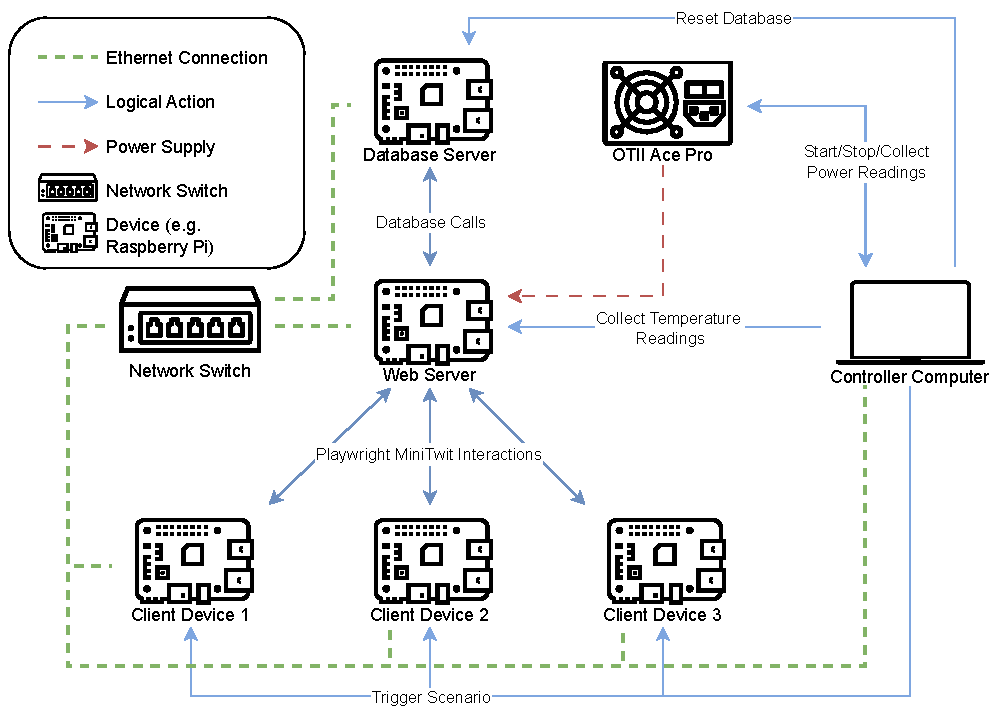
\includegraphics[width=.9\linewidth]{media/experiment/experiment-Setup.pdf}
    \caption{Overview of the experiment setup we use to measure the energy consumption of a MiniTwit implementation.}
    \label{fig:experiment-setup}
\end{figure}

The relevant hardware for our experiments consists of Raspberry Pi 4B's for Server (8GB RAM), Database (4GB RAM) and Client (8GB RAM) devices. All of them running Ubuntu Server 24.10 as OS. For the power supply and measuring device, we used the Otii Ace Pro.  

\subsubsection{Software Setup}

The software utilize containers in both the Database Server and Client Devices. The Web Server runs the MiniTwit implementations without containers to eliminate any uncertainties that the containers may cause in our measurements.

Using containers for the Database Server and Client Devices makes the development and deployment process easier, as development happens in the same environments as the actual experiment setup. Specifically, the client containers enabled simulating more clients using fewer devices, because each Client Device can run a container using just one of it's 4 cores and thereby run multiple client services in parallel. This made it possible for our experiment to run 12 client services using just 3 Client Devices. 

\subsubsection{The Experiment}
When talking about experiments, there is terminology we first need to cover.

\begin{itemize}
    \item \textbf{Experiment}: Consists of the steps related to running an experiment. These include starting and stopping power measurements, triggering scenarios, collecting temperature readings from the Web Server, etc.
    \item \textbf{Experiment Iteration}: Each experiment is repeated 5 times, where each of these repetitions is referred to as an iteration
    \item \textbf{Scenario}: The part of the experiment that simulates user interactions. It is implemented using Python scripts to interact with the MiniTwit application. The scenario consists of a specific set of actions.
\end{itemize}

An experiment starts by manually ensuring every device is connected and set up as specified in Figure \ref{fig:experiment-setup}, and the required software is running. Then the Controller Computer can execute the 5 experiment iterations.

Each iteration starts with a temperature reading from the Web Server's CPU. This is done to ensure that no experiment begins with an abnormal CPU temperature that could affect the results. Afterwards, it makes a call to the Otii to initiate the power measurement. The Controller Computer sends out calls to the 12 Client Services to start their scenario. After each of the 12 Client Services has finished the scenario, the Controller Computer finishes the Otii power measurement. Then it collects another temperature reading from the Web Server, to see how the CPU temperature changed during the experiment and ensure it remained within a reasonable range. Lastly, the Controller Computer collects the power draw readings from the Otii and saves them to a local CSV file.

The design idea behind the scenario is to ensure that we utilize the HTTP operations: POST, GET, and DELETE. Each of the operations is a part of the following stages of the scenario:

\begin{itemize}
    \item POST: When creating users or tweets, and when following a user, as that creates a follow-entry in the database. 
    \item GET: Navigating to any page that displays tweets results in a read operation.
    \item DELETE: When unfollowing a user.
\end{itemize}

The specific scenario can be found in the replication kit \cite{replication-kit-Karlsen_Landsgaard_Offenberg_Pedersen_2025}.

\subsection{Choice of Optimizations}
We decided to measure one or two optimizations for each implementation, depending on which were readily available. Additionally, for each implementation, a control experiment is run, with default optimizations. Which, from now on, is referred to as the default experiment. We decided on two types of optimizations, one related to the memory allocator (jemalloc) and one related to FDO, specifically JIT and PGO respectively.

Using PGO on an application requires profile data. For our experiments, we acquire the profile data by running a single data-collection experiment iteration with the default version of the specific implementation. The data-collection experiment iteration involves running the same scenario as all the other experiments; however, it is not included in the resulting power measurements. 

\subsection{Statistical Analysis}
To assess the significance of each experiment, we include p-values, which indicate the likelihood that the results are statistically different compared to the default experiment. A high p-value suggests no meaningful difference, while a value below 0.05 is considered statistically significant. 

We determine whether our data is normally distributed to identify the appropriate statistical test to use. For this, we run a Shapiro-Wilk test \cite{shapiro1965analysis}.

To determine statistical significance we use the parametric statistical test, Student's t-test \cite{student1908}, for the normally distributed data and the non parametric statistical test, Mann-Whitney U test \cite{mann1947test}, is used for the non-normal data. We do this to ensure the most accurate p-value for each experiment.

Each of these two tests also provides a statistical value: the t-statistic for the t-test and the U-statistic for the Mann-Whitney U test. These values are used to indicate the magnitude of the difference between the two compared datasets. A larger value means a larger difference. 

Additionally, we use the Pearson correlation coefficient to measure the linear relationship between execution time and power draw. It quantifies the strength of the correlation between the two variables and provides a value ranging from -1 to 1 \cite{sedgwick2012pearson}. Furthermore, it provides a p-value that must also be below 0.05 to be statistically significant. 

\subsubsection{Statistical Power Analysis}
We also conduct a power analysis to determine the minimum number of iterations necessary for our data to achieve a statistical power of 0.8, which indicates a 20\% chance of false negatives, and a significance level of 0.05, corresponding to the likelihood of false positives. We calculate the minimum number of sample iterations required for a given experiment and ensure an equal number of default iterations to facilitate a fair comparison. The equations we employ include Cohen's d \cite{cohen1988} for normally distributed data and a non-parametric power analysis \cite{noether1987} for non-normal datasets.
 
\end{document}
